
\cleardoublepage

\chapter{Experimental Setup}
\label{chapter:experiment}

The mapping system was evaluated at the Land Institute on a type of intermediate wheat grass, commonly referred to as Kernza.  The Land Institute is a research organization located in Salina, Kansas, focused on using perennial crops to develop sustainable farming practices.  The experiment, which was overseen by researcher Lee DeHaan, consisted of approximately 25,000 plants that were transplanted during the middle of October.  Details about how the field was setup, as well as different robot and camera settings, are discussed in this chapter. 

\begin{figure}[htb]
	\centering
    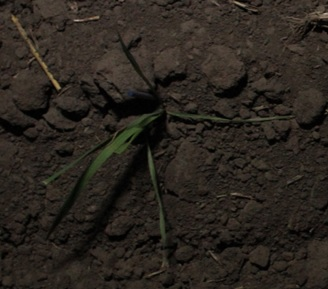
\includegraphics[height=3in]{figures/kernza_example.jpg}
    \caption[Kernza plant image]{Example of kernza seedling after transplanting. Image taken from the robot as it was driving through the field.}
    \label{figure:kernza_example}
\end{figure}

\section{Field Setup}
\label{section:field_setup}

A transplanter, shown in figure \ref{figure:transplanter}, was used to plant two rows a time.  The transplanter works by a series of six deposit cylinders rotating at a constant rate.  When a cylinder passes over the correct spot, its bottom flap is opened and the plant is ejected.  The yellow water tanks are used to automatically apply a small amount of water to the plant, and then the rolling wheels help press the soil down.  

The six deposit cylinders rotate so that each cylinder is spaced 12 inches apart.  Plants are placed in every other cylinder which results in 24 inches between successive plants.  The QR codes indicating the start of a new group are placed in the empty cylinders between two plants, which means the use of QR codes does not increase the overall size of the field. The spacing between the two rows on the transplanter was set to 36 inches, and this same spacing was used between each pass.  Therefore the entire field had consistent row-spacing. 

The plants were split into 97 individual rows, which were each roughly 180 meters long.  After the field was planted, the QR code marking the start and end of each row were manually placed.  The field contained 4581 QR codes.  Of these codes, 3619 corresponded to a plant grouping containing only a single plant.  The other 962 codes corresponded to plant groupings containing, on average, 25 plants.  

\begin{figure}[htb]
	\centering
    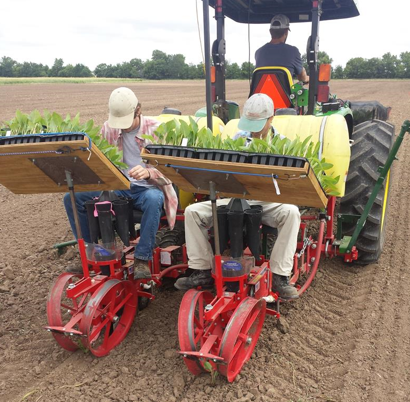
\includegraphics[width=3in]{figures/transplanter.jpg}
    \caption[Transplanter]{Two-row transplanter used for planting. Plants shown are a type of sunflower crop, not Kernza.}
    \label{figure:transplanter}
\end{figure}  

\section{Mapping Window}

An important decision is whether to map during the day or at night.  The biggest challenge of mapping during the day is the ability to provide consistent lighting.  Changes in scene lighting, for example between clouds and direct sun, can affect the color of plants and blue sticks and potentially cause under or over-exposure of QR codes.  Daytime lighting can be made more consistent by using a shade cover over the field of view of the images.  However, this depends on the sun being high enough in the sky for the shading to work, which limits the total amount of time images can be collected each day.  

The shade size can always be increased or placed at an angle to account for the sun angle, however this increases cost, design complexity and makes the platform more susceptible to wind gusts.  This time-limited window to collect images can be problematic due to the potential for storms to affect the QR codes.  Even if the QR codes are firmly planted in the ground and don't blow away, heavy rainfall can splash mud onto the codes decreasing the chance they'll be readable. 

Since the experiment was performed in October, when the sun only reaches a maximum altitude angle of 42 degrees, the decision was made to test the mapping process at night.  One disadvantage to mapping at night is the potential for the external lighting to attract insects which can fly into the camera's field of view.  From preliminary tests the LED bars did attract a few insects but not enough to negatively impact the usefulness of the images.

\begin{figure}[htb]
	\centering
    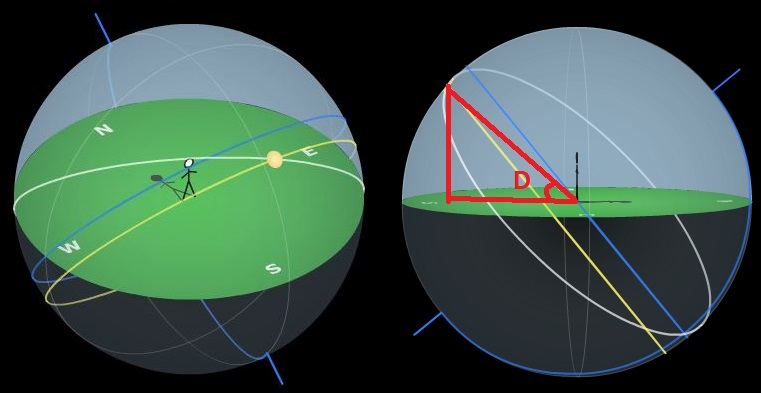
\includegraphics[width=5in]{figures/sun_angle2.jpg}
    \caption[Sun Angle]{Images showing sun altitude angle ($D$) at maximum point in the day for October 15th in Salina Kansas.}
    \label{figure:sun_angle}
\end{figure}  

\section{Camera Setup}

A critical step in ensuring the mapping process is robust is choosing the correct camera options.  Some of these options will vary in how they're determined between day and night-time mapping, because at night the available light is more restricted.  Since this experiment was performed at night, that is what is discussed here.

The first option selected is the shooting mode, as that defines what settings are available to change.  The preferred shooting mode is Manual as that will allow the exposure time, aperture, and sensitivity to be set to constant values.  Under controlled lighting conditions this will keep a consistent scene luminance and prevent any additional latency due to the camera calculating these settings before each image.

The maximum exposure time is determined based on the speed of the robot and maximum allowed translation in the QR codes.  If the exposure time is set too high the black and white squares making up the QR codes will start to blend together, and the code will be unreadable.  It was experimentally determined that an exposure time of 2.5 milliseconds, or 1/400 seconds, was sufficient for quality QR code images.

The aperture is set to a large diameter to maximize the amount of luminance since the exposure time is relatively short for the amount of light available.  However when the lens is fully open, an f-stop of f/2.8, the depth of field is noticeable reduced, and it becomes more difficult to keep the QR codes in focus as the camera height slightly varies as it moves through the field.  Therefore an f-stop of f/4 was chosen which provides a good trade-off between depth of field and luminance.  In addition, compared to f/2.8 an aperture of f/4 will have less noticeable lens effects such as distortion and vignetting, which results in higher quality images.  

The light sensitivity of the sensor, commonly specified as an \ac{iso} rating, is set last by inspecting the image in the field to achieve a desirable scene luminance.  Using the two LED bars per camera required an ISO of 1000.  If the ISO is set too high then sensor noise becomes significant.  If too high of an ISO is required, then the aperture can be made larger or the external light can be increased.  

The white-balance is set to a fixed setting chosen to match the same color of light as the LED bars, which is listed in the product description as 6000 Kelvins.  Many cameras offer both a Flash and Cloudy white balance which are both centered around 6000K.   Preliminary field tests indicate both options produce very similar results, so the Flash setting was used.  Auto-white balance mode should not be used as most images will not contain a QR code for reference, and as a result many images of plants will vary in chromacity. 

Finally, the image format is selected between raw and the \ac{jpg} format.  Raw images store the pixel readings directly from the sensor, thus no information from the exposed image is lost.  The \ac{jpg} format on the other hand typically merges adjacent pixels from the Bayer filter and applies a compression algorithm to reduce the file size.  Even though the compression algorithm produces image artifacts and reduces the quality of the QR codes, this does not reduce the effectiveness of the post-process pipeline. For the Canon 7D camera, raw image are around 15 megabytes (MB) larger and require a conversion to a bitmap format before being useful for post-processing.  This conversion requires approximately 5 to 10 seconds per image and adds a significant amount of additional processing time.  For these reason the \ac{jpg} format is used for mapping.

\begin{table}[htb]
    \begin{center}
    \caption[Camera Settings]{Camera settings for night-time mapping.}
    \begin{tabular}[c]{|c|c|}
        \hline
        Setting & Value \\
        \hline
        Camera Mode     & Manual        \\
        Aperture & f/4          \\
        Exposure & 1/400 seconds   \\
        ISO      & 1000  \\
        White Balance & 6000K \\
        Image Format & JPEG \\
        \hline
    \end{tabular}
    \label{table:camera_settings}
   \end{center}
\end{table}


\section{Robot Operation}

In section \ref{section:base_functionality} it was discussed that the robot can operate in either cruise control mode or a fully autonomous mode.  In this experiment the robot was used in cruise control mode, mainly because at the time there were not any tools available to view and edit the waypoints used by the robot.  When generating a set of waypoints from the transplanter path, the waypoints at the row ends need to be edited to prevent the robot from driving in too rough of field conditions, as well as to prevent from turning before the end of the row and running over plants.  Even though the robot was operating in cruise control mode, the path of the robot was recorded, and it's possible to have the robot retrace this path in autonomous mode.
